\documentclass[11pt]{article}
\usepackage{tikz}
\usepackage{amsmath}
\usepackage{mathtools}

%\usepackage{xfrac}
%\usepackage{hyperref}
%\usepackage[export]{adjustbox}
\def\checkmark{\tikz\fill[scale=0.4](0,.35) -- (.25,0) -- (1,.7) -- (.25,.15) -- cycle;} 
\usepackage{proj} 	% pull in style header
\usepackage{array}
\usepackage{sectsty}
\usepackage{soul}
\usepackage{float}
\restylefloat{table}

\lhead{ECE582: Formal Verification}


%----------------------------------------------------------------------------------------
%	TITLE SECTION
%----------------------------------------------------------------------------------------


\newcommand{\horrule}[1]{\rule{\linewidth}{#1}} % Create horizontal rule command with 1 argument of height

\title{	
\normalfont \normalsize 
\textsc{\LARGE Portland State University}\\[1.5cm] % Name of your university/college
\textsc{\Large Project 2}\\[0.5cm] % Major heading such as course name
\textsc{\large ECE582}\\[0.5cm] % Minor heading such as course title
%\textsc{Portland State University} \\ [25pt] % Your university, school and/or department name(s)
\horrule{1.2pt} \\[0.4cm] % Thin top horizontal rule
\huge Model Checking by NuSMV \\ % The assignment title
\horrule{1.2pt} \\[0.5cm] % Thick bottom horizontal rule
}

%----------------------------------------------------------------------------------------
%	AUTHOR SECTION
%----------------------------------------------------------------------------------------


\begin{document}\raggedright
\author{Erik Rhodes \and Jordan Fluth} % Your name
\maketitle % Print the title
\thispagestyle{empty}
\cfoot{\textit{Page \thepage { of} \pageref{LastPage}}}
\lhead{ECE582}
\chead{Project 2}
\rhead{Erik Rhodes \& Jordan Fluth}


\begin{figure}[h]\centering

\includegraphics[height=0.65\textwidth]{images/sat_intro.jpg}
	%\caption{Gameplay Block Diagram}
		\label{LED}
	\end{figure}
	
\newpage

% -------------------------PROJECT DELIVERABLES
%Part 1:
%Make circuit with 9 gates
%Draw circuit
%Make another identical copy C2. Prove C1=C2 by a Sat solver automatically.
%Download a SAT solver for satisfiability
%
%Part 2:
%Replace one gate with a different one
%Prove/disprove C1=C3 by a SAT solver automatically
%
%For the report, describe:
%Method to check equivalence by a SAT solver
%All CNF forms used in the proof
%All formulas and figures should be typed and drawn in software
%Detailed discussion of our derivation and solution



\section{Introduction} 
Talk about model checking


%\begin{figure}[h]\centering
%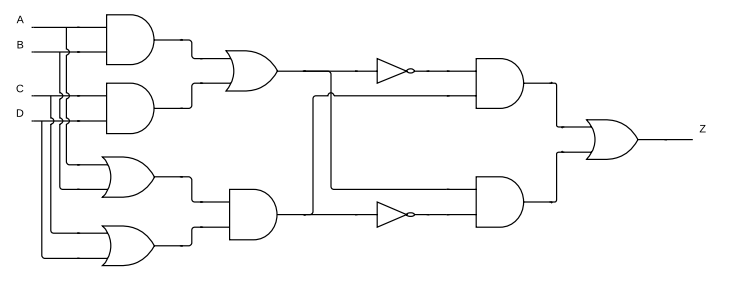
\includegraphics[height=0.45\textwidth]{images/c1.PNG}
%	\caption{Original Circuit}
%		\label{c1}
%	\end{figure}


%Symbols \And \wedge \vee \neg \to \gets \iff


\section{Combinational Lock}
	\subsection{NuSMV}
	\subsection{Added properties
	1. This property states that if the lock is open and it is not interrupted, it can remain open indefinitely.
		AG((open * ~up * ~down) → (open))

	2. This property states that a transition to state two can only happen under the required circumstances.
		AG(state=1 * ~open * down * ~up * position=21) → (state=2)

	3. This property states that if the lock is open and it is interrupted the the lock will close.
		AG((open * up * ~down) | (open * down * ~up)) → AX(~open)

	4. This property states that it is always possible for the lock to be closed.
		AG(EF(~open))

	5. This property states that the lock will not open by counting down to 15.
		AG(down * position=15) → (~open)
	}
	\subsection{Results}
	\subsection{Proofs
1. In the diagram, the red one mark the instance that shows this property is true. In state three the lock is open and if neither up, nor down is asserted then the lock continues to stay in state three and remain open.
2. In the diagram, the red two mark the instance that shows this property is true. In order for a transition to state two, you must have been in state one, the position of the count must be at 21, and you must have reached 21 by counting down.
3. In the diagram, the red three mark the instance that shows this property is true. In state three the lock is open, the only way to transition from state three, and thus close the lock, is by moving the position count up or down. If either of these happen there will be a transition to state zero and the lock will be closed.
4. In the diagram, the red four mark the instance that shows this property is true. In states zero, one, and two the lock is closed. State three is the only state in which the lock is open. Since there is a transition out of state three that is possible then there exist the possibility for the lock to be closed.
5. In the diagram, the red five mark the instance that shows this property is true. If in state two and counting up occurs there will be a transition to state zero. Therefore the lock will not be opened. 
	}
%\begin{figure}[h!]\centering
%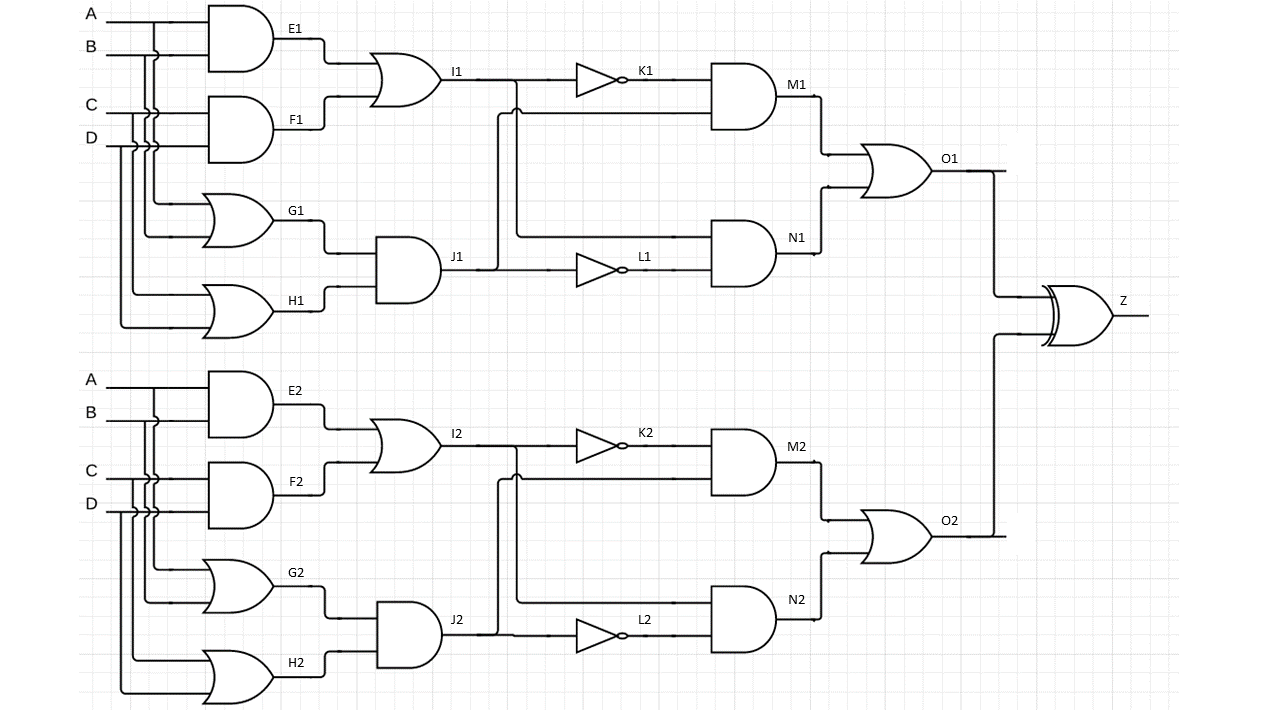
\includegraphics[height=0.55\textwidth]{images/c1c2.PNG}
%	\caption{Miter Circuit of C1 and C2}
%		\label{c2}
%	\end{figure}

\section{Kripke Structures} 

\subsection{Figure 1}
	\subsection{NuSMV}
	\subsection{Added properties
	1. This property states that from state three, the next transition must be to state four.
		AG(state=3) → AX(state=4)

	2. This property states that from state four, the next transition must be to state two.
		AG(state=4) → AX(state=2)

	3. This property states that from state five, it is possible to remain in state five indefinitely.
		AG(state=5) → EG(state=5)

	4. This property states that from state one, the next state cannot be five.
		AG(state=1) → ~EG(state=5)

	5. This property states that state three is reachable by state two or state five.
		AG(state=2 | state=5) → AX(state=3) 
	}
	\subsection{Results}
	\subsection{Proofs
1. In the diagram, the red one mark the instance that shows this property is true. If in state three there is only one possible transition. When in state three the next state will be state four.
2. In the diagram, the red two mark the instance that shows this property is true. If in state four there is only one possible transition. When in state four the next state will be state two.
3. In the diagram, the red three mark the instance that shows this property is true. If in state five one possible transition loops back to state five, therefore once you get in state five it is always possible to remain in state five.
4. In the diagram, the red four mark the instance that shows this property is true. If in state one, there is no transition to state five. Therefore, there is no path that leads from state one, to state five as the next state.
5. In the diagram, the red five mark the instance that shows this property is true. If in state two, or state five, there is a possible transition to state three.
	}
\subsection{Figure 2}
	\subsection{NuSMV}
	\subsection{Added properties
	1. This property states that from state six, the next transition must be to state seven.
		AG(state=6) → AX(state=7)

	2. This property states that from state three, the next transition must be to state four.
		AG(state=7) → AX(state=4)

	3. This property states that if in state three and the door is open then the next state, is state one.
		AG(state=3 * door) → AX(state=1)

	4. This property states that if in state five and a reset is signaled then the next state, is state three.
		AG(state=5 * reset) → AX(state=3)

	5. This property states that if in state four and it is cooking then it will remain in state four.
		AG(state=4 * cook) → AX(state=4)
	}
	\subsection{Results}
	\subsection{Proofs
1. In the diagram, the red one mark the instance that shows this property is true. If in state six there is only one possible transition. When in state six, the “warm up” signal is asserted, and the next state will be state seven.
2. In the diagram, the red two mark the instance that shows this property is true. If in state seven there is only one possible transition. When in state seven, the “start cooking” signal is asserted, and the next state will be state four.
3. In the diagram, the red three mark the instance that shows this property is true. If in state three and the “door open” signal is asserted, then the next state will be state one.
4. In the diagram, the red four mark the instance that shows this property is true.  If in state five and the “reset” signal is asserted, then the next state will be state three.
5. In the diagram, the red five mark the instance that shows this property is true.  If in state four and the “cooking” signal is asserted, then the next state will be state four.
	}
%\vspace{12pt}
%
%\begin{figure}[h]\centering
%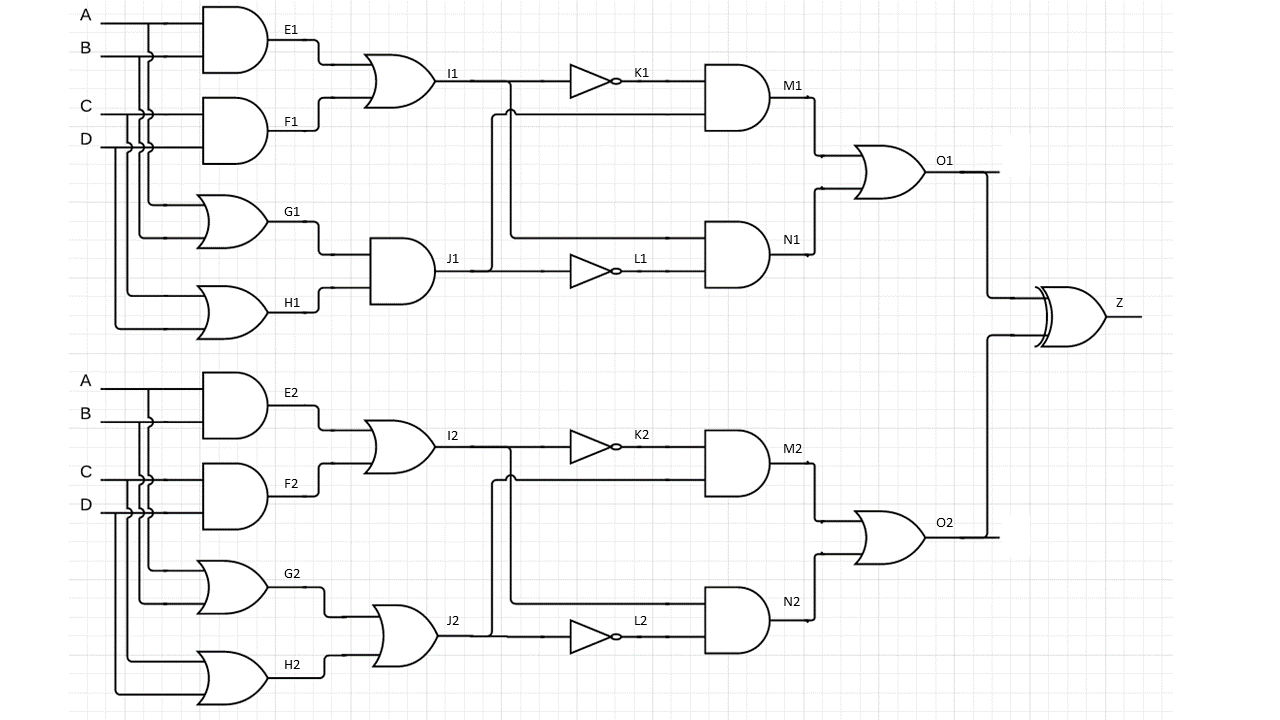
\includegraphics[height=0.5\textwidth]{images/c1c3.PNG}
%	\caption{Miter Circuit of C1 and C3}
%		\label{c3}
%	\end{figure}

\section{Equivalence Checking} 
\subsection{NuSMV}
\subsection{Results}
System Diameter.
Reachable states
Check AG(output=0)

%  
%\section{Results}
%Do we need to show any output from boolsat.com?
\end{document}
